\chapter{Introducción}

En esta Tesis se presenta una técnica novedosa de transmisión de datos en redes de tipo difusión, con énfasis en la privacidad, utilizando técnicas de espectro expandido.

%\section{Motivación}
Los sistemas de comunicacion ópticas han hecho posible las comunicaciones modernas. Tecnologías como Internet no son posibles sin una infraestructura óptica de comunicaciones de alta velocidad. 
La tasa de transmisión en enlaces individuales de la columna vertebral (\textit{backbone}) de Internet ha evolucionado recientemente de 10 Gbps, 100 Gbps y hasta 400 Gbps \cite{backbone} al momento de escribir este documento, utilizando técnicas tales como WDM (\textit{wavelength division multiplexing, multiplexación por división de longitud de onda}) y modulación coherente \cite{shieh2008coherent}, ambas tecnologías utilizadas para aumentar la tasa de transmisión de datos sobre la fibra óptica. 
Las redes de computadoras en general son redes de conmutación (\textit{packet switching)}, donde un ruteador procesa electrónicamente grupos de bytes denominados ``paquetes'' y los retransmite a los nodos de destino, enviando cada paquete individual a la interfaz de red correcta (Ver Fig. \ref{arch:simp}). Es un mecanismo eficiente en ancho de banda utilizado, pero requiere de una elevada cantidad de procesamiento.

\begin{figure}[!t]
  \centering
    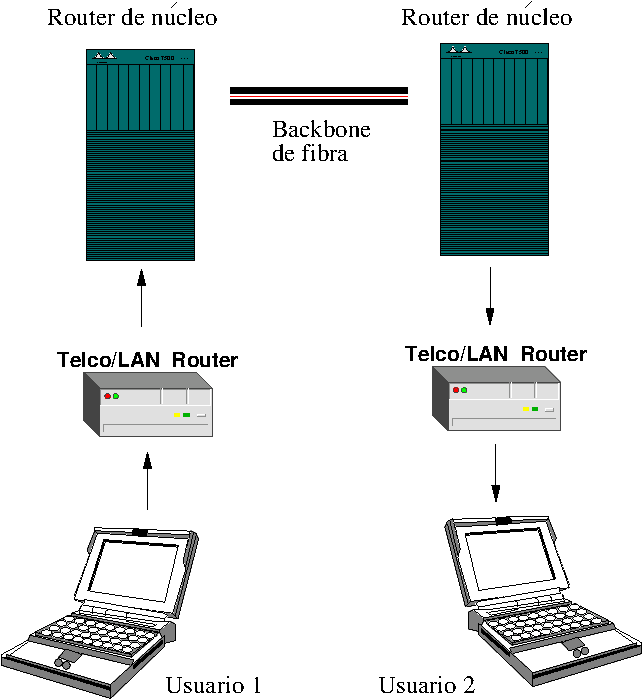
\includegraphics[width=4.0in]{graphs/internet.pdf}
    \caption{Simplificación del sistema de ruteo de Internet.}
    \label{arch:simp}
\end{figure}


Otro tipo de redes son las llamadas redes de difusión o \textit{broadcast}, que poseen algunas ventajas con respecto a las redes de conmutación de paquetes, tales como un sistema de ruteo mucho más simple que puede ser totalmente óptico, pero también tienen desventajas, tales como la necesidad de compartir el ancho de banda y problemas de seguridad inherentes al enviar la información a todos los nodos de la red. De esto se desprende que las redes de difusión deben generalmente contar con algún mecanismo que ofrezca privacidad, o de lo contrario su uso se restringe a aplicaciones que, o bien no requieren de ningún tipo de privacidad, o la privacidad se logra utilizando protocolos de alto nivel. Es sobre este tipo de redes donde se centra el aporte de esta Tesis.

Las redes de difusión no están limitadas al medio óptico. Pueden utilizar el medio electromagnético (por ejemplo, ondas de radio) o acústico (modems). Las comunicaciones de radio, por ejemplo, pueden ser espiadas por cualquier atacante que tenga una simple antena. Fue este problema en las comunicaciones de radio que impulsó la invención de técnicas criptográficas avanzadas en la segunda guerra mundial. Las comunicaciones de tipo difusión resultaron ser ideales para coordinar acciones bélicas en la segunda guerra, donde un emisor central podía impartir órdenes a toda el ejército utilizando ondas de radio, con la condicion obvia que solo aliados puedan participar de las comunicaciones. Esto motivó el desarrollo de los primeros dispositivos criptográficos tales como la máquina de Enigma \cite{kozaczuk1984enigma}, así como los primeros ataques matemáticos a la criptografía \cite{welchman1982hut}.

En tiempos modernos, las comunicaciones de tipo difusión fueron en gran parte desplazadas con respecto a las redes de conmutación de paquetes, especialmente en redes digitales de comunicaciones tales como Internet. Sin embargo existen nichos donde por motivos prácticos siguen siendo utilizadas redes de difusión casi exclusivamente, tal como la televisión y telefonía satelital. Gran parte de la complejidad de estos sistemas se debe a los sistemas de seguridad que deben contener para prevenir fraudes y pérdida de privacidad \cite{hanas1981addressable}.

Continuando con esta línea de investigación, los problemas de seguridad en las redes de difusión motivaron el diseño que utiliza un medio óptico o acústico donde la privacidad esté implementada en la capa física, sin requerir ningún tipo de soporte de software o del sistema operativo. El objetivo es crear una VLAN \textit{(Virtual Local Area Network, red local virtual)} donde cada cliente pueda realizar comunicaciones de datos privadas con cualquier otro, sin revelar ninguna información a los demás.

Esto apunta a fomentar el desarrollo de sistemas economicos de FTTH (\textit{Fiber to the Home}) donde un diseño de red de difusión óptica con seguridad a nivel físico permitiría utilizar componentes pasivos de muy bajo costo (ver Fig. \ref{arch:ftth}). Si bién es sencillo realizar un enlace punto-a-punto óptico o acústico utilizando cualquier algoritmo de encriptación simétrica estandard, la creación de una verdadera red, con múltiples clientes y canales punto-a-multipunto no tiene una solución clara hasta el momento.

Luego de un período de exploración de posibles diseños y soluciones se desarrolló un sistema de comunicaciones, que luego de calculada su eficiencia y apoyados los resultados por medio de simulaciones numéricas, se procedió a su implementación como prototipo, primero sobre un medio acústico y finalmente sobre un medio óptico. 
En el medio acústico se utilizaron dispositivos informáticos comunes, tales como laptops y teléfonos celulares del tipo smartphone, utilizando los mismos micrófonos y parlantes de los mismos para establecer una red VLAN acústica. 
Para la implementación sobre medio óptico se utilizó una placa de desarrollo FPGA, un dispositivo capaz de procesar las altas tasas de transferencia del medio óptico.
Esta Tesis documenta las experiencias obtenidas en el diseño, implementación y medición del algoritmo implementado sobre varios dispositivos y medios diferentes.

\begin{figure}[!t]
  \centering
    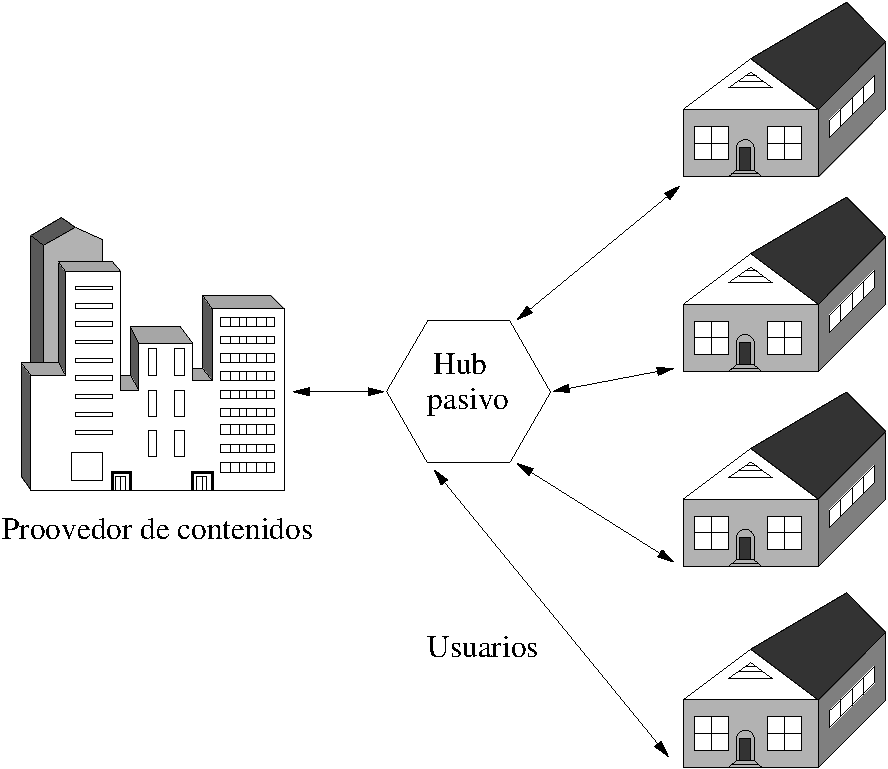
\includegraphics[width=3.5in]{graphs/ftth.pdf}
    \caption{Sistema FTTH propuesto. Un proovedor de contenidos (Ej. Datos, TV, o telefonía, lo que se denomina ``triple-play'') utiliza un concentrador de muy bajo costo para conectarse directamente a los usuarios finales por medio de una conexión de fibra óptica.}
    \label{arch:ftth}
\end{figure}

\section{Contribuciones}

A continuación citaremos las contribuciones que esta Tesis ha realizado a la comunidad, en la forma de artículos o patentes:

\textbf{Altas velocidades de transferencia en fibra óptica utilizando FPGAs de bajo costo. } \textit{A. A. Ortega, V. A. Bettachini, D.F. Grosz, J. I. Alvarez-Hamelin - Congreso de Microelectrónica Aplicada 2010 BsAs}: En este artículo se documenta una técnica para utilizar FPGAs (\textit{Field Programmable Gate Array}) con transceptores ópticos normales, a mayor velocidad que la documentada. Utilizando los circuitos internos del transceptor independientes de los circuitos de la FPGA que lo contiene, es posible generar señales de pruebas de hasta 12 Gbps, con una longitud máxima de patrón de 11 bits individualmente controlables. Estos patrones de prueba tienen aplicaciones tanto para la caracterización de canales como para la experimentación con pulsos Laser o eléctricos.

\

\textbf{ Point-to-point and Point-to-multipoint CDMA Access Network with Enhanced Security} \textit{ A. A. Ortega, V. A. Bettachini, J. I. Alvarez-Hamelin,  D.F. Grosz, Advanced Photonics 2011 Congress - Access Networks and In-house CommunicationsAccess Networks and In-house Communications, OSA Technical Digest, Optical Society of America}: Se presenta la primera versión de la red segura, funcionando sobre un medio de fibra óptica y con un aprovechamiento del medio del 13\%. Se propone una diseño de red segura en la capa física, utilizando la tecnica de time-hopping CDMA, y logrando comunicaciones criptográficamente seguras punto-a-punto y punto-a-multipunto. Una implementación con topología es en estrella es analizada, capáz de soportar hasta 128 usuarios situados hasta a 20 Km de distancia del nodo central. Se utiliza el algoritmo LDPC (\textit{(Low Density Parity Check)}) como parte del sistema de corrección de errores. Se demuestra la feasibilidad del sistema mediante simulaciones numéricas.

\

\textbf{Hamming-weight minimisation coding for CDMA optical access networks with enhanced security} \textit{ A. A. Ortega, V. A. Bettachini, J. I. Alvarez-Hamelin, D.F. Grosz, Future Generation Communication Technology (FGCT), 2012}: Este artículo se muestra un diseño similar al anterior, pero con una modificación en la pila de corrección de errores que eleva el aprovechamiento del medio al 33\%. Esto se logra eliminando la etapa de corrección LDPC y reemplazándola por una corrección de errores realizada directamente en el Bloom Filter encriptado, que es optimizado por el algoritmo de minimización de peso de Hamming. Utilizando un diseño en estrella, el sistema continua soportando 128 usuarios simultaneos situados hasta a 20 km de distancia del nodo central. Hay que destacar que estas características se cumplen utilizando un hub central pasivo. Utilizando un repetidor o hub central activo, las distancias pueden ser mayores.


\

\textbf{Encrypted CDMA Audio Network.} \textit{ A. A. Ortega, V. A. Bettachini, P. I. Fierens, y J. I. Alvarez-Hamelin.  Journal of Information Security - 2014}: Este artículo se centra en la implementación del protocolo sobre el medio acústico, ahondando en la sincronización, implementación y mediciones sobre distintos dispositivos móbiles, tales como celulares y laptops, demostrando que si bien la modulación necesaria para la creación de un canal Z tiene muy baja eficiencia espectral, es altamente compatible, resistente a interferencias y puede ser utilizada para transmitir de manera privada a distancias prácticas por la mayoría de los dispositivos testeados.


%\section{Patentes}

Se presentaron los siguientes pedidos de patentes en oficinas de patentes nacionales (Argentina) (patente asignada) e internacionales (EU) (patente en trámite al momento de escritura de esta Tesis):

\textbf{DISPOSITIVO Y MÉTODO PARA TRANSMISIÓN SEGURA DE DATOS SOBRE CANALES Z MEDIANTE CDMA (AR084155B1)}\textit{José Ignacio ALVAREZ HAMELIN, Victor Alexis BETTACHINI, and Alfredo ORTEGA. PCT, 12 2012. (Asignada)}

\textbf{Device and Method for the Secure Transmission of Data over Z-Channels Using CDMA (P11104EPPC)}\textit{José Ignacio ALVAREZ HAMELIN, Victor Alexis BETTACHINI, and Alfredo ORTEGA. EPO, Julio 2014. (En trámite)}


%\section{Contribución}


\section{Organización de este documento}

En el primer capítulo ``Introducción'' se presentan las motivaciones, contribuciones y algunas definiciones. Se describe en alto nivel la estructura de la Tesis.

En el segundo capítulo ``Fundamentos y Estado del arte'' se presenta un resumen de todas las tecnologías utilizadas, así como las definiciones necesarias.

El tercer capítulo ``Sistema propuesto: teoría y simulaciones'' se discuten las decisiones de diseño y se simula de manera numérica el sistema completo.

El cuarto capítulo ``Resultados experimentales: medios de transmisión óptica y acústica'' describe los detalles de implementación y mediciones en medios ópticos y acústicos. Se detalla el diseño de alto nivel de los generadores de frame en una FPGA para el protocolo en el medio óptico y la implementación en software que precisan los dispositivos móviles que utilizarán el medio acústico. Se detallan, también, los algoritmos de sincronización desarrollados, necesarios para las mediciones y para la creación de un prototipo funcional.

Finalmente, en el quinto capítulo, ``Conclusiones'', se finaliza la Tesis presentando las conclusiones obtenidas fruto de la investigación e implementación de los algoritmos y sistemas propuestos, y se sugieren posibles mejoras o aportes específicos a realizar en el futuro.
